\documentclass[12pt, a4paper, oneside]{article}
\usepackage{graphicx}
\usepackage{arial}
\renewcommand{\familydefault}{\sfdefault}
\usepackage[T1]{fontenc}
\usepackage[polish]{babel}
\usepackage[utf8]{inputenc}
\usepackage{lmodern}
\usepackage[left=2cm,right=2cm,top=2cm,bottom=2cm]{geometry}
\selectlanguage{polish}
\usepackage{booktabs, multicol, multirow}
\usepackage{longtable}
\begin{document}
\section{Wstęp}
\indent\indent W obwodach RLC, czyli składających się z rezystorów, cewek oraz kondensatorów zasilanych prądem zmiennym może wystąpić zjawisko rezonansu elektromagnetycznego. Prąd w obwodzie gwałtownie osiąga wtedy maksimum. Ma to miejsce, gdy $X_L + X_C = 0$, gdzie $X_L =\omega L$ - reaktancja cewki, a $X_C = -\frac{1}{\omega C}$ - reaktancja kondensatora. Z tej równości można wyznaczyć:\\
\begin{equation}
f_{r} = \frac{1}{2\pi\sqrt{LC}}.
\end{equation}
Dla $f_{r}$ amplituda prądu osiąga maksymalną wartość:
\begin{equation}
I=\frac{U_0}{Z}=\frac{U_0}{R+j\omega L+\frac{1}{j\omega C}}=\frac{U_0}{R}.
\end{equation}
Wynika to z prawa Ohma oraz faktu, że impedancja dla częstotliwości rezonansowej zależy jedynie od części rzeczywistej, czyli rezystancji. Łatwo więc zauważyć, że krzywa rezonansowa powinna osiągać większą amplitudę wraz ze spadkiem rezystancji.
\begin{figure}[h!]
\centering
\caption{Schemat wykorzystanego układu pomiarowego}
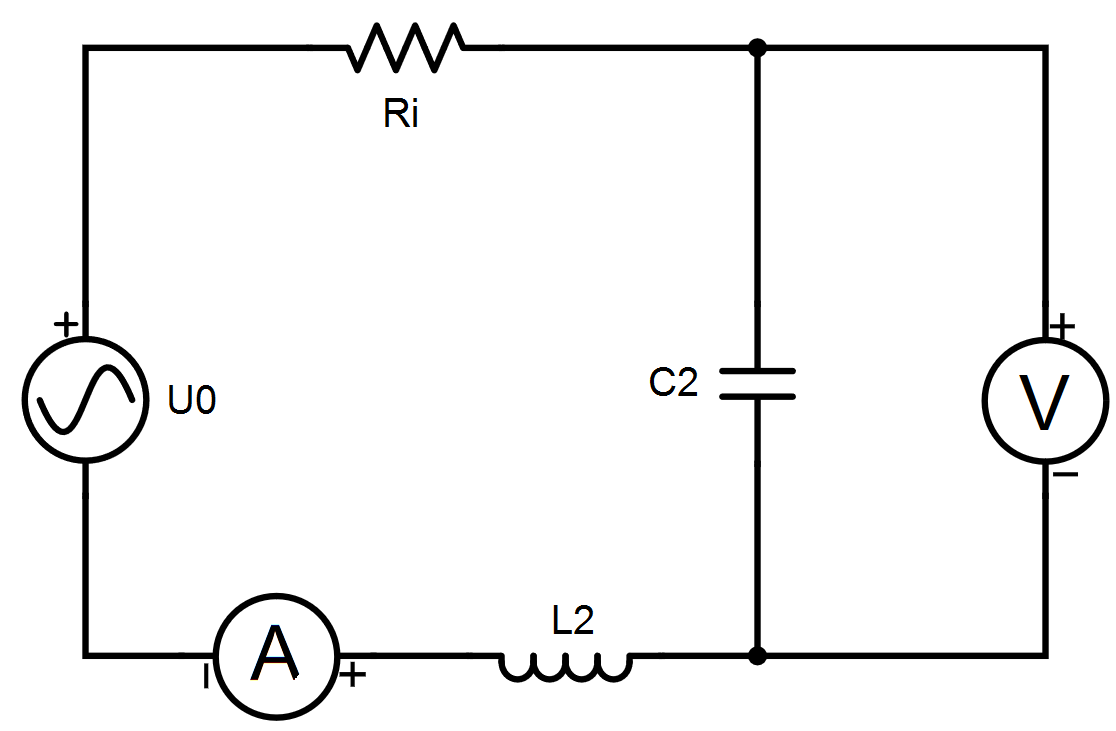
\includegraphics[scale=0.35]{f1.png}
\end{figure}
\\\indent Dobroć układu - stosunek wymuszonych drgań rezonansowych do analogicznej amplitudy w~obszarze częstotliwości nierezonansowych:
\begin{equation}
Q=\frac{f_{r}}{\Delta f}=\frac{U_C}{U_0},
\end{equation}
gdzie:\\
- $\Delta f$ - szerokość krzywej rezonansowej w połowie jej wysokości,\\
- $U_C$ - napięcie na kondensatorze.
\section{Wykorzystane wzory}
Niepewność napięcia źródła
\begin{equation}
u(U_0) = 3\%~rdg
\end{equation}
Niepewność pomiaru rezystancji
\begin{equation}
u(R_i) = 0.5\%~rdg + 1~dgt
\end{equation}
Niepewność pomiaru pojemności
\begin{equation}
u(C) = 5\%~rdg + 10~dgt
\end{equation}
Niepewność pomiaru częstotliwości
\begin{equation}
u(f) = 1\%~rdg + 1~dgt
\end{equation}
Niepewność pomiaru prądu
\begin{equation}
u(I) = 2.5\%~rdg + 3~dgt
\end{equation}
Niepewność pomiaru napięcia
\begin{equation}
u(U) = 0.8\%~rdg + 1~dgt
\end{equation}
Wyznaczana pojemność kondensatora
\begin{equation}
C = \frac{1}{(2\pi f_r)^2L}
\end{equation}
Niepewność wyznaczanej pojemności kondensatora
\begin{equation}
u_C(C)=\frac{1}{2\pi^2}\sqrt{[\frac{u(L)}{2f_r^2L^2}]^2+[\frac{u(f_r)}{f_r^3L}]^2}
\end{equation}
Wyznaczana (szacowana z wykresu) dobroć układu
\begin{equation}
Q=\frac{U_C}{U_0}(=\frac{f_r}{\Delta f})
\end{equation}
Niepewność wyznaczanej dobroci układu
\begin{equation}
u_C(Q)=\sqrt{[\frac{u(U_C)}{U_0}]^2+[\frac{U_C}{U_0^2}u(U_0)]^2}
\end{equation}
\section{Przykładowe obliczenia}
Niepewność napięcia źródła
\begin{center}
$u(3) = 0.8\%\cdot3=0.09~[V]$
\end{center}
Niepewność pomiaru rezystancji
\begin{center}
$u(55.7) = 0.5\%\cdot55.5+0.1=0.38~[\Omega]$
\end{center}
Niepewność pomiaru pojemności
\begin{center}
$u(100) = 5\%\cdot + 10=15~[nF]$
\end{center}
Niepewność pomiaru częstotliwości
\begin{center}
$u(1000) = 1\%\cdot 1000 + 1 = 11~[Hz]$
\end{center}
Niepewność pomiaru prądu
\begin{center}
$u(0.190) = 2.5\%\cdot 0.190 + 0.003=0.035$
\end{center}
Niepewność pomiaru napięcia
\begin{center}
$u(3.053) = 0.8\%\cdot3.053+0.001=0.026$
\end{center}
\clearpage
\section{Opracowanie pomiarów}
\begin{table}[h!]
  \centering
  \caption{Zmierzone bezpośrednio parametry obwodu RLC}
    \begin{tabular}{|c|c|c|c|}\hline
    $i$ & $1$ & $2$ & $3$ \\\hline
    $R_i~[\Omega]$ & 55.70 & 111.50 & 275.9 \\\hline
    $u(R_i)~[\Omega]$ & 0.38 & 0.66 & 1.5 \\\hline
    $C_2~[nF]$ & \multicolumn{3}{|c|}{100 $\pm$ 15} \\\hline
    $L_2~[mH]$ & \multicolumn{3}{|c|}{33.0 $\pm$ 3.3} \\\hline
    $U_0~[V]$ & \multicolumn{3}{|c|}{3.00 $\pm$ 0.09} \\\hline
    \end{tabular}%
  \label{tab:addlabel}%
\end{table}%
% Table generated by Excel2LaTeX from sheet 'Arkusz1'
\begin{table}[h!]
  \centering
  \caption{Wyniki pomiarów dla obwodu z opornikiem R$_1$}
    \begin{tabular}{|c|c|c|c|c|c|}\hline
    $f~[Hz]$ & $u(f)~[Hz]$ & $I~[mA]$ & $u(I)~[mA]$ & $U~[V]$ & $u(U)~[V]$ \\\hline
    100 & 2 & 0.190 & 0.035 & 3.053 & 0.026 \\\hline
    500 & 6 & 1.040 & 0.056 & 3.108 & 0.026 \\\hline
    1000 & 11 & 2.220 & 0.086 & 3.279 & 0.028 \\\hline
    1500 & 16 & 3.72 & 0.13 & 3.630 & 0.031 \\\hline
    2000 & 21 & 5.97 & 0.18 & 4.360 & 0.036 \\\hline
    2500 & 26 & 10.15 & 0.29 & 5.780 & 0.048 \\\hline
    2600 & 27 & 11.49 & 0.32 & 6.230 & 0.051 \\\hline
    2700 & 28 & 13.09 & 0.36 & 6.790 & 0.056 \\\hline
    2800 & 29 & 15.05 & 0.41 & 7.470 & 0.061 \\\hline
    2900 & 30 & 17.46 & 0.47 & 8.280 & 0.068 \\\hline
    3000 & 31 & 20.36 & 0.54 & 9.240 & 0.075 \\\hline
    3100 & 32 & 23.62 & 0.63 & 10.290 & 0.084 \\\hline
    3200 & 33 & 26.88 & 0.71 & 11.260 & 0.092 \\\hline
    3300 & 34 & 29.44 & 0.77 & 11.920 & 0.097 \\\hline
    3400 & 35 & 30.6 & 0.8 & 12.030 & 0.098 \\\hline
    3500 & 36 & 30.23 & 0.79 & 11.580 & 0.094 \\\hline
    3600 & 37 & 28.70 & 0.75 & 10.750 & 0.087 \\\hline
    3700 & 38 & 26.6 & 0.7 & 9.77 & 0.08 \\\hline
    3800 & 39 & 24.40 & 0.64 & 8.800 & 0.072 \\\hline
    3900 & 40 & 22.29 & 0.59 & 7.920 & 0.065 \\\hline
    4000 & 41 & 20.39 & 0.54 & 7.130 & 0.059 \\\hline
    4100 & 42 & 18.7 & 0.5 & 6.430 & 0.053 \\\hline
    4200 & 43 & 17.16 & 0.46 & 5.830 & 0.048 \\\hline
    4300 & 44 & 15.82 & 0.43 & 5.300 & 0.044 \\\hline
    4400 & 45 & 14.7 & 0.4 & 4.84 & 0.04 \\\hline
    4500 & 46 & 13.62 & 0.38 & 4.440 & 0.037 \\\hline
    5000 & 51 & 9.95 & 0.28 & 3.001 & 0.026 \\\hline
    5500 & 56 & 7.74 & 0.23 & 2.203 & 0.019 \\\hline
    6000 & 61 & 6.29 & 0.19 & 1.701 & 0.015 \\\hline
    6500 & 66 & 5.26 & 0.17 & 1.364 & 0.012 \\\hline
    \end{tabular}%
  \label{tab:addlabel}%
\end{table}%
\begin{center}
Maksymalny prąd I = (30.6 $\pm$ 0.8) A przy częstotliwości f = (3400 $\pm$ 35) Hz.\\
Napięcie na kondensatorze dla tej częstotliwości wynosi U = (12.030 $\pm$ 0.098) V.\\
Dobroć układu Q = 4.01 $\pm$ 0.13.
\end{center}
\clearpage
% Table generated by Excel2LaTeX from sheet 'Arkusz1'
\begin{table}[h]
  \centering
  \caption{Wyniki pomiarów dla obwodu z opornikiem R$_2$}
    \begin{tabular}{|c|c|c|c|c|c|}\hline
    $f~[Hz]$ & $u(f)~[Hz]$ & $I~[mA]$ & $u(I)~[mA]$ & $U~[V]$ & $u(U)~[V]$ \\\hline
    100 & 2 & 0.190 & 0.035 & 3.053 & 0.026 \\\hline
    500 & 6 & 1.040 & 0.056 & 3.105 & 0.026 \\\hline
    1000 & 11 & 2.210 & 0.086 & 3.265 & 0.028 \\\hline
    1500 & 16 & 3.68 & 0.13 & 3.6 & 0.03 \\\hline
    2000 & 21 & 5.79 & 0.18 & 4.240 & 0.035 \\\hline
    2500 & 26 & 9.31 & 0.27 & 5.340 & 0.044 \\\hline
    2600 & 27 & 10.30 & 0.29 & 5.650 & 0.047 \\\hline
    2700 & 28 & 11.41 & 0.32 & 5.990 & 0.049 \\\hline
    2800 & 29 & 12.64 & 0.35 & 6.360 & 0.052 \\\hline
    2900 & 30 & 13.98 & 0.38 & 6.760 & 0.056 \\\hline
    3000 & 31 & 15.37 & 0.42 & 7.150 & 0.059 \\\hline
    3100 & 32 & 16.74 & 0.45 & 7.500 & 0.061 \\\hline
    3200 & 33 & 17.56 & 0.47 & 7.770 & 0.064 \\\hline
    3300 & 34 & 18.90 & 0.51 & 7.920 & 0.065 \\\hline
    3400 & 35 & 19.44 & 0.52 & 7.910 & 0.065 \\\hline
    3500 & 36 & 19.55 & 0.52 & 7.740 & 0.063 \\\hline
    3600 & 37 & 19.27 & 0.52 & 7.450 & 0.061 \\\hline
    3700 & 38 & 18.7 & 0.5 & 7.070 & 0.058 \\\hline
    3800 & 39 & 17.92 & 0.48 & 6.630 & 0.055 \\\hline
    3900 & 40 & 17.05 & 0.46 & 6.190 & 0.051 \\\hline
    4000 & 41 & 16.13 & 0.44 & 5.760 & 0.048 \\\hline
    4100 & 42 & 15.22 & 0.42 & 5.340 & 0.044 \\\hline
    4200 & 43 & 14.35 & 0.39 & 4.950 & 0.041 \\\hline
    4300 & 44 & 13.52 & 0.37 & 4.590 & 0.038 \\\hline
    4400 & 45 & 12.71 & 0.35 & 4.250 & 0.035 \\\hline
    4500 & 46 & 11.99 & 0.33 & 3.950 & 0.033 \\\hline
    5000 & 51 & 9.21 & 0.27 & 2.793 & 0.024 \\\hline
    5500 & 56 & 7.34 & 0.22 & 2.101 & 0.018 \\\hline
    6000 & 61 & 6.06 & 0.19 & 1.645 & 0.015 \\\hline
    6500 & 66 & 5.11 & 0.16 & 1.328 & 0.012 \\\hline
    \end{tabular}%
  \label{tab:addlabel}%
\end{table}%
\begin{center}
Maksymalny prąd I = (19.55 $\pm$ 0.52) A przy częstotliwości f = (3500 $\pm$ 36) Hz.\\
Napięcie na kondensatorze dla tej częstotliwości wynosi U = (7.740 $\pm$ 0.063) V.\\
Dobroć układu Q = 2.580 $\pm$ 0.081.
\end{center}
\clearpage
% Table generated by Excel2LaTeX from sheet 'Arkusz1'
\begin{table}[h]
  \centering
  \caption{Wyniki pomiarów dla obwodu z opornikiem R$_3$}
    \begin{tabular}{|c|c|c|c|c|c|}\hline
    $f~[Hz]$ & $u(f)~[Hz]$ & $I~[mA]$ & $u(I)~[mA]$ & $U~[V]$ & $u(U)~[V]$ \\\hline
    100 & 2 & 0.19 & 0.035 & 3.052 & 0.026 \\\hline
    500 & 6 & 1.03 & 0.056 & 3.086 & 0.026 \\\hline
    1000 & 11 & 2.16 & 0.084 & 3.190 & 0.027 \\\hline
    1500 & 16 & 3.45 & 0.12 & 3.383 & 0.029 \\\hline
    2000 & 21 & 5.01 & 0.16 & 3.663 & 0.031 \\\hline
    2500 & 26 & 6.83 & 0.21 & 3.960 & 0.033 \\\hline
    2600 & 27 & 7.21 & 0.22 & 3.998 & 0.033 \\\hline
    2700 & 28 & 7.57 & 0.22 & 4.120 & 0.034 \\\hline
    2800 & 29 & 7.91 & 0.23 & 4.150 & 0.035 \\\hline
    2900 & 30 & 8.23 & 0.24 & 4.170 & 0.035 \\\hline
    3000 & 31 & 8.51 & 0.25 & 4.170 & 0.035 \\\hline
    3100 & 32 & 8.76 & 0.25 & 4.150 & 0.035 \\\hline
    3200 & 33 & 8.97 & 0.26 & 4.120 & 0.034 \\\hline
    3300 & 34 & 9.11 & 0.26 & 4.070 & 0.034 \\\hline
    3400 & 35 & 9.21 & 0.27 & 4.000 & 0.033 \\\hline
    3500 & 36 & 9.25 & 0.27 & 3.920 & 0.033 \\\hline
    3600 & 37 & 9.26 & 0.27 & 3.820 & 0.032 \\\hline
    3700 & 38 & 9.21 & 0.27 & 3.710 & 0.031 \\\hline
    3800 & 39 & 9.13 & 0.26 & 3.5 & 0.03 \\\hline
    3900 & 40 & 9.01 & 0.26 & 3.417 & 0.029 \\\hline
    4000 & 41 & 8.86 & 0.26 & 3.291 & 0.028 \\\hline
    4100 & 42 & 8.69 & 0.25 & 3.163 & 0.027 \\\hline
    4200 & 43 & 8.5 & 0.25 & 3.036 & 0.026 \\\hline
    4300 & 44 & 8.3 & 0.24 & 2.910 & 0.025 \\\hline
    4400 & 45 & 8.09 & 0.24 & 2.786 & 0.024 \\\hline
    4500 & 46 & 7.88 & 0.23 & 2.667 & 0.023 \\\hline
    5000 & 51 & 6.83 & 0.21 & 2.138 & 0.019 \\\hline
    5500 & 56 & 5.89 & 0.18 & 1.728 & 0.015 \\\hline
    6000 & 61 & 5.11 & 0.16 & 1.418 & 0.013 \\\hline
    6500 & 66 & 4.46 & 0.15 & 1.182 & 0.011 \\\hline
    \end{tabular}%
  \label{tab:addlabel}%
\end{table}%
\begin{center}
Maksymalny prąd I = (9.25 $\pm$ 0.27) A przy częstotliwości f = (3600 $\pm$ 37) Hz.\\
Napięcie na kondensatorze dla tej częstotliwości wynosi U = (3.820 $\pm$ 0.032) V.\\
Dobroć układu Q = 1.27 $\pm$ 0.04.
\end{center}
\clearpage
\begin{figure}[h]
\centering
\caption{Wykres zależności amplitudy prądu w funkcji częstotliwości dla układu z kondensatorem C$_2$ i cewką L$_2$ przy wyborze różnych wartości oporu}
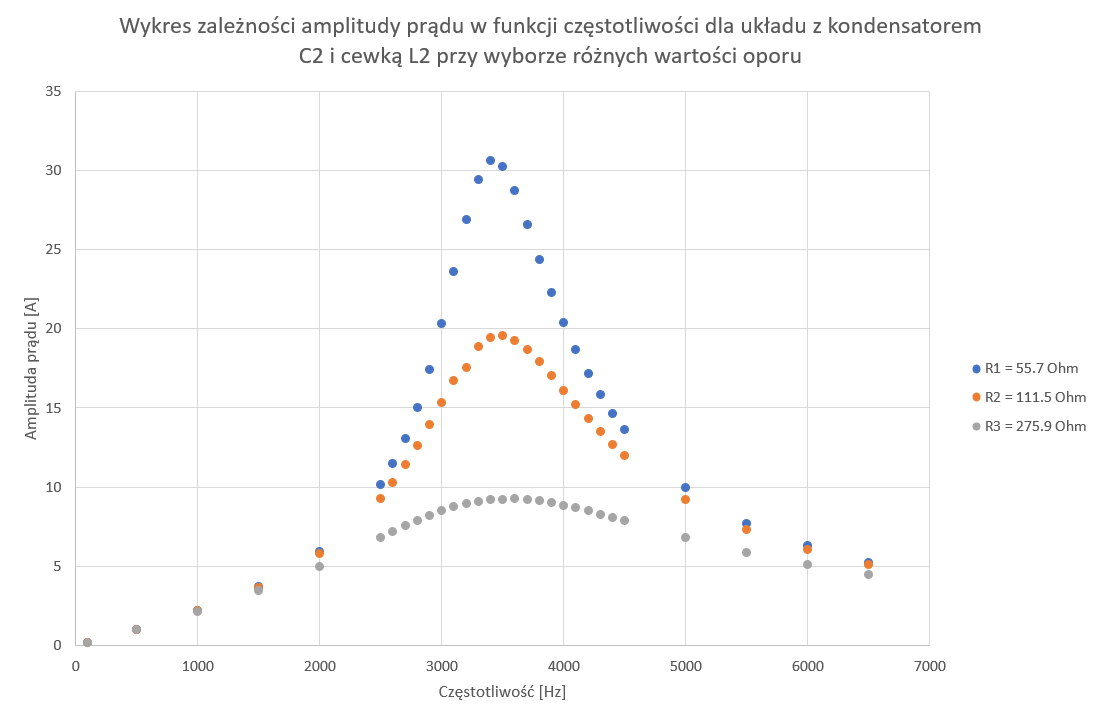
\includegraphics[scale=0.45]{f2.png}
\end{figure}
\section{Wnioski}
\begin{itemize}
\item Częstotliwość rezonansowa układu wynosi f$_r$ = (3 500.00 $\pm$ 20.79) Hz
\item Zmierzona bezpośrednio pojemność kondensatora C$_2$ wynosi C = (100 $\pm$ 15) nF.
\item Wyznaczona pośrednio pojemność kondensatora C$_2$ wynosi C = (103 $\pm$ 11) nF.
\item Pojemności wyznaczona pośrednio oraz zmierzona bezpośrednio są zbieżne, jednak metoda bezpośrednia w tym wypadku daje rezultat obarczony niepewnością większą o 4 nF.
\item Wyznaczona dobroć układu z opornikiem:
\begin{itemize}
\item R$_1$: Q = 4.01 $\pm$ 0.13,
\item R$_2$: Q = 2.580 $\pm$ 0.081,
\item R$_3$: Q = 1.27 $\pm$ 0.04.
\end{itemize}
\item Szacowana dobroć układu z opornikiem:
\begin{itemize}
\item R$_1$: Q = 2.33,
\item R$_2$: Q = 1.6,
\item R$_3$: Q = 1.1.
\end{itemize}
Wartości oszacowane obarczone są dużą niepewnością, która może mocno fałszować wynik.
\end{itemize}
\end{document}